
\chapter{Basic robust statistics}
\label{chap:stats}

Many measures of location, scale, \Index{skewness} and \Index{kurtosis} or
heaviness of the tails have been proposed and studied in the statistical
literature. The present chapter is devoted to the comparison of the
(asymptotic) \Index{Gaussian efficiency} and robustness performance of three
different classes of estimators: (i) “classic” estimators, based on (centered)
moments of the distribution $F_n$; (ii) estimators built from specific
quantiles of the distribution; (iii) estimators defined on the basis of
pairwise comparisons or combinations of the observations. In addition, we will
discuss robust test of normality and robust boxplots.

\section{Robust estimation of location}
\label{sec:stats:location}
\index{subject}{location estimators|(textbf}

There is apparent consensus in applied statistics about the fact that the
sample \Index{mean} and the sample \Index{median} are two complementary location estimators:
the mean is very efficient in case of Gaussian (i.e.\ normally distributed)
data but fragile to outliers (and problematic in case of highly asymmetric
data) while the median is very robust (and meaningful in case of asymmetry) but
rather inefficient. Both are extensively used in practice. Let us briefly
recall their respective properties and introduce two other frequently used
location estimators.

\subsection{The mean and the $\alpha$-trimmed mean}
\index{subject}{mean|(textbf}\index{subject}{$\alpha$-trimmed mean|(textbf}

The \emph{mean} corresponds to the functional $\mu = \mu(F) =
\int_{-\infty}^\infty x \dif F(x)$;                                              \todo{Comment on integrals: Why not 
                                                                                $\int x f(x)\dif x$? Maybe show somewhere that
                                                                                $\int f(x) \dif x = \int \dif F(x)$}
its empirical counterpart is $\mu_n = \mu(F_n) = \frac{1}{n} \sum_{i=1}^n x_i$.
It is well known that this location estimator is the most efficient estimator
for Gaussian data; its asymptotic variance is $\stsc{ASV}(\mu, F) =
\sigma^2$, where $\sigma^2$ denotes the variance of the distribution $F$
(taking $F = \Phi$, the standard normal distribution, we have $\stsc{ASV}(\mu,
\Phi) = 1$). Unfortunately, the mean lacks robustness. Indeed, one single
outlying observation can move this estimator towards an arbitrarily large (absolute)
value: its asymptotic breakdown point $\epsilon^*(\mu, F)$ is equal to 0.
Likewise, its influence function is unbounded, leading to an infinite
gross-error sensitivity: $\stsc{IF}(x; \mu, F) = x - \mu$ (see \citealp[p.
25]{wilcox:2005}). Figure~\ref{fig:stat:IF_loc}a shows the influence function of
$\mu$ under the standard normal distribution.                                   \todo{Why “under the standard normal distribution”?
                                                                                Isn't the influence function always the 
                                                                                same irrespective of $F$?}


\begin{figure}[h!]
    \centering
    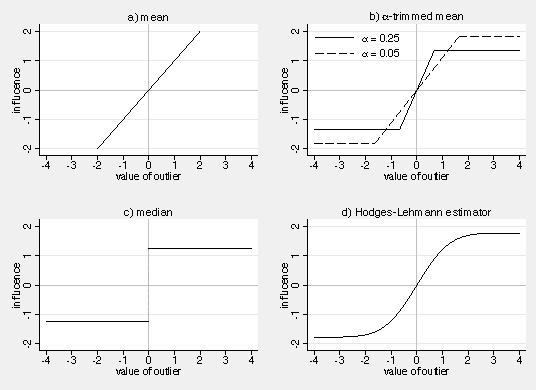
\epsfig{file=eps/3/1,width=.9\textwidth}
    \caption{Influence functions of $\mu$, $\mu^{0.25}$, $\mu^{0.05}$, $Q_{0.5}$, and $\stsc{HL}$ under the standard normal distribution}
    \label{fig:stat:IF_loc}
\end{figure}

A simple and classical way to “robustify” the sample mean consists in
discarding a certain proportion $\alpha$ ($0\leq\alpha<0.5$) of the smallest
and of the biggest observations in the sample. This leads to the
$\alpha$-\emph{trimmed mean} defined by
\[
    \mu_n^\alpha =\frac{1}{n - 2\lfloor \alpha n \rfloor}
        \sum_{i = \lfloor \alpha n \rfloor + 1}^{n - \lfloor \alpha n \rfloor} x_{(i)}
\]
where $\lfloor x \rfloor$ denotes the integer part of $x$ and $x_{(i)}$ is the
$i$th order statistic (the observation at the $i$th position in the list of
sorted observations in ascending order). Note that the sample mean $\mu_n$ is
a special case of the $\alpha$-trimmed mean $\mu_n^\alpha$ corresponding
to $\alpha = 0$. The functional associated with this location estimator is
\[
    \mu^\alpha(F) = \frac{1}{1-2\alpha} \int_{Q_\alpha}^{Q_{1-\alpha}} x \dif F(x)
\]
where $Q_\alpha = F^{-1}(\alpha)$ and $Q_{1-\alpha} = F^{-1}(1-\alpha)$ are the
$\alpha$ and $(1-\alpha)$ quantiles of distribution $F$. 

The influence function of this functional has the advantage to be bounded. If
$F$ is symmetric, then
\[
    \stsc{IF}(x; \mu^\alpha, F) = 
    \begin{cases}
        \frac{1}{1-2\alpha}\left(F^{-1}(\alpha) - \mu\right)   & \text{if $x<F^{-1}(\alpha)$} \\
        \frac{1}{1-2\alpha}(x - \mu)                           & \text{if $F^{-1}(\alpha)\leq x\leq F^{-1}(1-\alpha)$} \\
        \frac{1}{1-2\alpha}\left(F^{-1}(1-\alpha) - \mu\right) & \text{if $x>F^{-1}(1-\alpha)$}
    \end{cases}
\]
(see, e.g., \citealp{staudte:sheather:1990}). As an example, see Figure
\ref{fig:stat:IF_loc}b for the influence functions of $\mu^{0.05}$ and
$\mu^{0.25}$ under the standard Gaussian distribution $\Phi$.

Moreover, the asymptotic breakdown point of $\mu^\alpha$ is equal to
$100\alpha\%$. Clearly, hence, the proportion $\alpha$ of trimming appears as a
parameter allowing to choose the level of robustness of the trimmed mean. 
Of course, this gain in robustness goes hand in hand with a loss in efficiency.
Yet, this loss is not as large as one may fear. Using the fact that
\[
    \stsc{ASV}(\mu^\alpha, F) = \int_{-\infty}^\infty \stsc{IF}(x; \mu^\alpha, F)^2 \dif F(x)
\]
we obtain, for example,                                                         \todo{How did you compute these numbers? 
                                                                                Are there closed form solutions?}
\[
    \stsc{ASV}(\mu^{0.05}, \Phi) \approx 1.0263 \qquad
    \stsc{ASV}(\mu^{0.10}, \Phi) \approx 1.0604 \qquad
    \stsc{ASV}(\mu^{0.25}, \Phi) \approx 1.1952
\]
for the standard normal distribution. Hence, the asymptotic Gaussian relative
efficiency of $\mu^\alpha$ with respect to the mean, defined as
$\stsc{ASV}(\mu, \Phi) / \stsc{ASV}(\mu^\alpha, \Phi) = 1 /
\stsc{ASV}(\mu^\alpha, \Phi)$, reaches 97\% for $\alpha = 0.05$, 94\% for
$\alpha = 0.10$, and, despite the fact that half of the sample is discarded,
84\% for $\alpha = 0.25$.
\index{subject}{mean|)}\index{subject}{$\alpha$-trimmed mean|)}

\subsection{The median}
\index{subject}{median|(textbf}

The \emph{median}---the quantile of order 0.5---corresponds to the
functional $Q_{0.5}(F) = F^{-1}(0.5)$. Its empirical version $Q_{0.5; n}$ is
simply the sample median $F_n^{-1}(0.5)$, typically computed as
\[
    Q_{0.5;n} = 
    \begin{cases}
        x_{((n+1)/2)}                       & \text{if $n$ is odd}\\[1ex]
        \frac{x_{(n/2)} + x_{(n/2 + 1)}}{2} & \text{if $n$ is even}
    \end{cases}
\]
where $x_{(i)}$ again denotes the $i$th order statistic among $x_1, \dots,
x_n$.

The median performs better than the mean from the robustness point of view
(see, e.g., \citealp[p.\ 56 and 59]{staudte:sheather:1990}). First of all, its
influence function is given by
\[
    \stsc{IF}(x; Q_{0.5}, F) =
    \begin{cases}
        -\frac{1}{2f\left(F^{-1}(0.5)\right)} & \text{if $x < F^{-1}(0.5)$}\\[1ex]
        0                                     & \text{if $x = F^{-1}(0.5)$}\\[1ex]
        \frac{1}{2 f\left(F^{-1}(0.5)\right)} & \text{if $x > F^{-1}(0.5)$}
    \end{cases}
\]
where $f$ is the density function associated with $F$. In particular, as
displayed in Figure~\ref{fig:stat:IF_loc}c, $\stsc{IF}(x; Q_{0.5}, \Phi) =
\sign(x) \sqrt{\pi/2}$ for standard Gaussian data, since $f\left(\Phi^{-1}(0.5)\right) = \sqrt{\pi/2}$. This
influence function is bounded, leading to a bounded gross-error sensitivity, but
it has a discontinuity at $x = 0$.                                              \todo{Say why the discontinuity is a problem.}
Furthermore, the asymptotic breakdown point of
the median is equal to 50\% and is thus higher than the asymptotic breakdown
point of the $\alpha$-trimmed mean, regardless of the value of $\alpha$.

Finally, the asymptotic variance of the median is given as
\[
    \stsc{ASV}(Q_{0.5}, F) = \frac{1}{4 f\left(F^{-1}(0.5)\right)^2}
\]
Hence, relative Gaussian efficiency compared to the mean is
equal to 
\[
    \frac{\stsc{ASV}(\mu, \Phi)}{\stsc{ASV}(Q_{0.5}, \Phi)} 
    = \frac{1}{\pi/2} = \frac{2}{\pi} \approx 64\%
\]
\index{subject}{median|)}

\subsection{The Hodges-Lehmann estimator}
\index{subject}{Hodges-Lehmann estimator|(textbf}

\citet{hodges:lehmann:1963} have introduced an alternative location estimator
that has the advantage of a bounded, continuous and smooth influence
function, but also a high asymptotic Gaussian relative efficiency with respect
to the sample mean. The \emph{Hodges-Lehmann estimator} at the sample 
$\stmat{X}_n$ is defined by                                                    \todo{Can't we type
                                                                                $\stsc{HL}_n = \displaystyle\med_{i<j}\textstyle\left(\frac{x_i+x_j}{2}\right)$?
                                                                                This would seem easier to understand to me.
                                                                                Also, why only $i<j$? Why not all possible combinations (even including $i=j$)?}
\[
    \stsc{HL}_n = \med\left\{\frac{x_i+x_j}{2}; i<j \right\}
\]
It is the empirical version of the functional $\stsc{HL} = \stsc{HL}(F)$,
which is defined as the median of the distribution of $(X+Y)/2$, where $X$ and
$Y$ are i.i.d.\ random variables of distribution $F$.

For symmetric $F$, the influence function of $\stsc{HL}$ is given as
                                                                                \todo{I use $f(x)^2$ instead of 
                                                                                $f^2(x)$. I know the latter is often used in 
                                                                                stats literature, but to me the former much is
                                                                                clearer.}
\[
    \stsc{IF}(x; \stsc{HL}, F) = \frac{2 F(x-\mu) - 1}{2 \int_{-\infty}^\infty f(y)^2 \dif y}
\]
Figure~\ref{fig:stat:IF_loc}c presents the influence function for standard Gaussian
data. It illustrates that outliers have a bounded influence. Also note that the \todo{The original just said that the sensitivity
                                                                                depends on the smoothness of $F$ without saying 
                                                                                why this is relevant. I thus added some text. Please
                                                                                check, whether it is ok.}
sensitivity of the Hodges-Lehmann estimator depends on the smoothness of $F$.
Hence, the \Index{local-shift sensitivity} is small as long as the data have a  
smooth distribution function.

Because $\stsc{HL}$ combines the robust properties of the \Index{median} with the
efficiency properties of averaging, it performs well for a variety of
distributions. Based on (\ref{eq:ASV}) we obtain
\[
    \stsc{ASV}(\stsc{HL}, F) = \frac{1}{12} \left(\frac{1}{\int_{-\infty}^\infty f(y)^2 \dif y}\right)^2
\]
For example, for standard Gaussian date, $\stsc{ASV}(\stsc{HL}, \Phi) =
\pi/3 = 1.0472$. Hence, the asymptotic efficiency of the Hodges-Lehmann
estimator relative to the \Index{mean} is equal to $3/\pi \approx 95\%$ at the
normal distribution. Moreover, the Hodges-Lehmann estimator reaches a relative
efficiency with respect to the mean of at least 86\% for any symmetric
distribution (see, for example, \citealp[p. 120-121]{staudte:sheather:1990}).
Compared to the median, the Hodges-Lehmann estimator has a higher Gaussian
efficiency (95\% vs. 64\%) but a lower asymptotic breakdown point (29\% vs.
50\%).

\index{subject}{Hodges-Lehmann estimator|)}

\subsection{M estimate of location}

\alert{[What about \stsc{M} estimators???]}

\subsection{Summary}


Table \ref{tab:stat:location} summarizes the different properties of the four
location estimators. From the perspective of a good balance between high
Gaussian efficiency and a high breakdown point, the Hodges-Lehmann estimator
appears to perform particularly well.

\begin{table}[h!]
    \centering
    \caption{Characteristics of the four location estimators}
    \label{tab:stat:location}
    \begin{tabular}{lcccc}
        \toprule
        Estimator
        & Class  
        & \subtab{c}{Gaussian\\ efficiency}
        & \subtab{c}{Asymptotic\\ breakdown\\ point} 
        & \subtab{c}{Bounded\\ influence\\ function}
        \\\midrule
        mean $\mu_n$                            & moment   & 100\% &  0\%          & no
        \\\addlinespace
        $\alpha$-trimmed mean $\mu_n^{\alpha}$  & moment   & 
            \subtab{l}{$\alpha=0.05$: 97\%\\ $\alpha=0.10$: 94\%\\ $\alpha=0.25$: 84\%} 
                                                                   & $100\alpha\%$ & yes
        \\\addlinespace
        median $Q_{0.5;n}$                      & quantile & 64\%  & 50\%          & yes
        \\\addlinespace
        Hodges-Lehmann $\stsc{HL}_n$            & pairwise & 95\%  & 29\%          & yes
        \\\bottomrule
    \end{tabular}
\end{table}
\index{subject}{location estimators|)}


\section{Robust estimation of scale\label{subsec:scale}}
\index{subject}{scale estimators|(textbf}


\subsection{The standard deviation}
\index{subject}{standard deviation|(textbf}

The classic statistic to estimate the scale parameter of a distribution 
is the \emph{standard deviation} $\sigma_n$, 
corresponding to the functional 
\[
    \sigma = \sigma(F) = \sqrt{\int_{-\infty}^\infty (x-\mu)^2 \dif F(x)}
\]
At sample $\stmat{X}_n$, $\sigma_n$ is typically computed as                   \todo{I changed this to the usual 
                                                                                $1/(n-1)$ variant; if we use the 
                                                                                $1/n$ version we need to explain why.}
\[
    \sigma_n = \sigma(F_n) = \sqrt{\frac{1}{n-1} \sum_{i=1}^n (x_i-\mu_n)^2}
\]
with $\mu_n$ as defined above. The standard deviation is the most efficient
estimator of the scale parameter $\sigma$ in case of Gaussian data (note that
$\stsc{ASV}(\sigma, \Phi)=0.5$).                                               \todo{Show why $\stsc{ASV}(\sigma, \Phi)=0.5$}
However, just like the mean, the standard
deviation is very fragile to outliers. Its influence function, given as
\[
    \stsc{IF}(x; \sigma, F) = \frac{1}{2\sigma} \left(x^2 - 2\mu x + \mu^2 - \sigma^2\right)
\]
is unbounded and its asymptotic breakdown point is equal to 0\% (e.g.,
\citealp[p. 1275]{rousseeuw:croux:1993}). The influence function for standard
Gaussian data, given as $\stsc{IF}(x; \sigma, \Phi) = \frac{1}{2} (x^2 - 1)$,
is displayed in Figure~\ref{fig:stat:IF_scale}a.

\index{subject}{standard deviation|)}


\begin{figure}[h!]
    \centering
    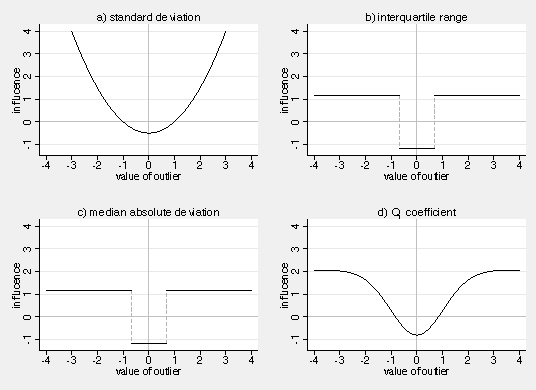
\epsfig{file=eps/3/2,width=.9\textwidth}
    \caption{Influence functions of $\sigma$, $\stsc{IQR}_c$, $\stsc{MAD}$ and $Q$ under the standard normal distribution}
    \label{fig:stat:IF_scale}
\end{figure}


\subsection{The interquartile range}
\index{subject}{interquartile range|(textbf}

A common alternative scale measure, defined on the basis of quantiles, is the
\emph{interquartile range}
\[
    \stsc{IQR}= Q_{0.75} - Q_{0.25}
\]
where $Q_{0.25}$ and $Q_{0.75}$ are the first and third quartiles of
distribution $F$. Instead of $\stsc{IQR}$ one frequently uses the
\emph{corrected interquartile range} $\stsc{IQR}_c$ defined as
\[
    \stsc{IQR}_c = d \cdot \stsc{IQR}
\]
where $d$ is a constant chosen to make the estimator $\stsc{IQR}_{c;n}$
\Index[Fisher consistency]{Fisher-consistent} for the scale parameter of the
underlying distribution. For example, for a Gaussian distribution, use $d =
1 / \left(\Phi^{-1}(0.75) - \Phi^{-1}(0.25)\right) \approx 0.7413$ to make the
corrected interquartile range a consistent estimator for the usual scale
parameter $\sigma$.

The influence function of the interquartile range is bounded, but discontinuous
(see, for example, \citealp[p. 35–36]{wilcox:2005}). It is given as
\[
    \stsc{IF}(x; \stsc{IQR}, F) =
    \begin{cases}
        \frac{1}{f\left(F^{-1}(0.25)\right)} - C & \text{if $x < F^{-1}(0.25)$}\\[1ex]
        -C                                       & \text{if $F^{-1}(0.25) \leq x \leq F^{-1}(0.75)$}\\[1ex]
        \frac{1}{f\left(F^{-1}(0.75)\right)} - C & \text{if $x > F^{-1}(0.75)$}
    \end{cases}
\]
where 
\[
    C = \frac{1}{4} \left[\frac{1}{f\left(F^{-1}(0.25)\right)} + \frac{1}{f\left(F^{-1}(0.75)\right)}\right]
\]

Note that $\stsc{IF}(x; \stsc{IQR}_c, F) = d \cdot \stsc{IF}(x;
\stsc{IQR}, F)$. Figure~\ref{fig:stat:IF_scale}b displays the influence
function of $\stsc{IQR}_c$ for standard Gaussian data. Like the two quartiles
$Q_{0.25}$ and $Q_{0.75}$, $\stsc{IQR}$ and $\stsc{IQR}_c$ have an
asymptotic breakdown point equal to 25\%. This gain in robustness with respect
to the standard deviation is accompanied by a high loss in Gaussian
efficiency. Specifically, $\stsc{ASV}(\stsc{IQR}_c, \Phi) = 1.3605$ so that      \todo{Give details about $\stsc{ASV}(\stsc{IQR}_c, \Phi)$. How is it computed?}
the asymptotic Gaussian efficiency of the corrected interquartile range with
respect to the standard deviation is equal to $\stsc{ASV}(\sigma, \Phi) /
\stsc{ASV}(\stsc{IQR}_c, \Phi) = 0.5/1.3605 \approx 37\%$.

\index{subject}{interquartile range|)}

\subsection{The median absolute deviation}
\index{subject}{median absolute deviation|(textbf}

Another robust alternative is the \emph{median absolute deviation}, whose
empirical version is defined as
\[
    \stsc{MAD}_n = d \cdot \med_i\left|x_i-\med_j x_j\right|
\]
That is, the median absolute deviation is equal to the (rescaled) median of the
absolute deviations from the median of the variable of interest. For Gaussian
distributions, we need to set $d = 2 / \left(\Phi^{-1}(0.75) -
\Phi^{-1}(0.25)\right) \approx 1.4826$ to make $\stsc{MAD}_n$
Fisher-consistent for the scale parameter $\sigma$.

The functional corresponding to $\stsc{MAD}_n$ is 
\[
    \stsc{MAD} = \stsc{MAD}(F) = d \cdot G_{F}^{-1}(0.5)
\]
where $G_{F}$ is the distribution function of $|X-Q_{0.5}(F)| = |X-F^{-1}(0.5)|$ 
with $X$ as a random variable of distribution $F$. In other
words, $\stsc{MAD}$ is equal to $d$ times the median of the distribution
associated with $|X-Q_{0.5}(F)|$, the magnitude of the difference between $X$
and its median.

The median absolute deviation may appear more attractive than the
interquartile range for certain purposes. It has the same asymptotic
Gaussian efficiency as the corrected interquartile range, but performs better
in terms of robustness (e.g., \citealp[p. 1273–1274]{rousseeuw:croux:1993}):
Its asymptotic breakdown point is as high as 50\%. The influence function 
of $\stsc{MAD}$ is given as $d \cdot \stsc{IF}(x; G_{F}^{-1}(0.5), F)$ with
\[
    \stsc{IF}(x; G_{F}^{-1}(0.5), F)
    = \frac{\sign\left(|x-F^{-1}(0.5)| - G_{F}^{-1}(0.5)\right) - C \cdot \sign\left(x-F^{-1}(0.5)\right)}
    {2 \left[f\left(F^{-1}(0.5) + G_{F}^{-1}(0.5)\right) + f\left(F^{-1}(0.5) - G_{F}^{-1}(0.5)\right)\right]}
\]
where
\[
    C = \frac{f\left(F^{-1}(0.5) + G_{F}^{-1}(0.5)\right) - f\left(F^{-1}(0.5) - G_{F}^{-1}(0.5)\right)}
    {f\left(F^{-1}(0.5)\right)}
\]
(see, e.g., \citealp{wilcox:2005}). In particular, under the standard Gaussian
distribution (with $F=\Phi$ and $f=\phi$), we have                              \todo{Is it only for Gaussian data 
                                                                                that the IF for IQR and MAD is the same,
                                                                                or is this true for any symmetric 
                                                                                distribution?}
\[
    \stsc{IF}(x; \stsc{MAD}, \Phi) 
    = 1.4826 \cdot\frac{\sign\left(|x| - \Phi^{-1}(0.75)\right)}
                       {4\,\phi\left(\Phi^{-1}(0.75)\right)}
\]
which is displayed in Figure \ref{fig:stat:IF_scale}c.                          \todo{In Rousseeuw/Croux the IF of MAD is closer to that one of Q; check that...}


Despite its good robustness properties, $\stsc{MAD}$ is primarily useful for
\emph{symmetric} distributions. In fact, the $\stsc{MAD}$ corresponds to
finding the symmetric interval around the median that contains 50\% of the data
(50\% of the probability mass), which does not appear to be a very sensible
approach for asymmetric distributions. The interquartile range does not have
this restriction, as the quartiles need not be equally far away from the median.

\index{subject}{median absolute deviation|)}


\subsection{The $Q_n$ coefficient}

Finally, a very interesting but relatively unknown scale estimator is the
$Q_n$ statistic introduced by \citet{rousseeuw:croux:1993}:
\[
    Q_n =   d\cdot \{|x_i-x_j|; i<j\}_{(k)}
\]
where $d$ is a constant factor allowing $Q_n$ to be a Fisher-consistent
estimator for the scale parameter of the underlying distribution $F$ and $k =
\binom{h}{2} \approx \binom{n}{2}/4$, with $h = \lfloor n/2\rfloor + 1$ ($h$ is
roughly half the number of observations). In other words, if we omit the
constant $d$, the statistic $Q_n$ corresponds approximately to the 0.25
quantile of the $\binom{n}{2}$ distances $|x_i-x_j|$, $i<j$. Fisher-consistency for the 
scale parameter $\sigma$ at Gaussian distributions can be achieved by setting
$d = 1/\left(\sqrt{2}\Phi^{-1}(5/8)\right) \approx 2.2191$.                     \todo{In Rousseeuw/Croux the value is 2.2219,
                                                                                 which seems to be an error.}

The functional counterpart of $Q_n$ is 
\[
    Q = Q(F) = d\cdot H_{F}^{-1}(0.25)
\]
where $H_{F}$ is the distribution function of $|X-Y|$ with $X$ and $Y$ being two
independent random variables of distribution $F$. Note that $Q(F_n)$ is not
exactly the same as $Q_n$, where we take an order statistic among $\binom{n}{2}$
elements instead of $n^2$ elements, but asymptotically this makes no difference.

The scale estimator $Q_n$ has globally better properties than the previous
scale estimators we have presented. Like the $\stsc{MAD}$, it has an asymptotic
breakdown point equal to 50\%. Yet, unlike the $\stsc{MAD}$, $Q_n$ is not
slanted towards symmetric distributions. Moreover, its influence function is
not only bounded, but also smooth:                                              \todo{I use numerical integration to obtain 
                                                                                the value of the denominator (used for the 
                                                                                graph and for the computation of the efficiency).
                                                                                Is there also a closed-form solution?}
\[
    \stsc{IF}(x; Q, F) = d\cdot \frac{0.25 - F(x+d^{-1}) + F(x-d^{-1})}{\int_{-\infty}^\infty f(y+d^{-1}) \dif F(y)}
\]
Figure~\ref{fig:stat:IF_scale}d displays the influence function of $Q_n$ for 
standard Gaussian data.                                                         

Finally, $Q_n$ is asymptotically more efficient than the median absolute
deviation under Gaussian distributions. In particular, numerical integration of
$\int_{-\infty}^\infty \stsc{IF}(x;Q,\Phi)^2 \dif \Phi(x)$ yields
$\stsc{ASV}(Q,\Phi) \approx .6089$, corresponding to an asymptotic Gaussian        \todo{I get 0.6089, not 0.6077.}
relative efficiency with respect to the standard deviation of
$\stsc{ASV}(\sigma, \Phi) / \stsc{ASV}(Q, \Phi) \approx 0.5/.6089 \approx 82\%$,
which is surprisingly high.

\todo{The following output shows my computations. Results should     be precise (e.g., they do not change if I increase the number of              integration points to 100000). This is just for you. It will be removed       later on.}
\begin{stlog}
. use Star.dta, clear
{\smallskip}
. regress log_intensity log_temperature
{\smallskip}
      Source {\VBAR}       SS           df       MS      Number of obs   =        47
\HLI{13}{\PLUS}\HLI{34}   F(1, 45)        =      2.08
       Model {\VBAR}  .664593334         1  .664593334   Prob > F        =    0.1557
    Residual {\VBAR}  14.3463934        45  .318808743   R-squared       =    0.0443
\HLI{13}{\PLUS}\HLI{34}   Adj R-squared   =    0.0230
       Total {\VBAR}  15.0109868        46  .326325799   Root MSE        =    .56463
{\smallskip}
\HLI{14}{\TOPT}\HLI{64}
log_intensity {\VBAR}      Coef.   Std. Err.      t    P>|t|     [95\% Conf. Interval]
\HLI{14}{\PLUS}\HLI{64}
log_tempera{\tytilde}e {\VBAR}  -.4133041   .2862575    -1.44   0.156    -.9898562     .163248
        _cons {\VBAR}   6.793468   1.236516     5.49   0.000     4.302998    9.283939
\HLI{14}{\BOTT}\HLI{64}
{\smallskip}

\end{stlog}

\subsection{Summary}

To conclude, Table \ref{tab:stat:scale} summarizes the different properties of the
presented estimators of scale. As is evident, the $Q_n$ coefficient has superior
properties in terms of robustness and efficiency compared to the other robust 
estimators.

\begin{table}[h!]
    \centering
    \caption{Characteristics of the four scale estimators}
    \label{tab:stat:scale}
    \begin{tabular}{lcccc}
        \toprule
        Estimator
        & Class  
        & \subtab{c}{Gaussian\\ efficiency}
        & \subtab{c}{Asymptotic\\ breakdown\\ point} 
        & \subtab{c}{Bounded\\ influence\\ function}
        \\\midrule
        standard deviation $\sigma_n$              & moment   & 100\% &  0\% & no
        \\\addlinespace
        interquartile range $\stsc{IQR}_n$       & quantile & 37\%  & 25\% & yes
        \\\addlinespace
        median absolute deviation $\stsc{MAD}_n$ & quantile & 37\%  & 50\% & yes
        \\\addlinespace
        $Q_n$ coefficient                 & pairwise & 82\%  & 50\% & yes
        \\\bottomrule
    \end{tabular}
\end{table}

\index{subject}{scale estimators|)}


\section{Robust estimation of skewness}
\label{subsec:skewness}
\index{subject}{skewness estimators|(textbf}

\subsection{The Fisher coefficient}
\index{subject}{Fisher coefficient|(textbf}

As far as skewness is concerned, the most classic estimator is the \emph{Fisher
coefficient}. Given sample $\stmat{X}_n$ the Fisher coefficient is defined as
\[
    \gamma_{1; n} = \frac{1}{n} \sum_{i=1}^n\left(\frac{x_i - \mu_n}{\sigma_n}\right)^{3}
\]
with $\mu_n$ and $\sigma_n$ as the sample \Index{mean} and the 
\Index{standard deviation}. This estimator is associated with the functional
\[
    \gamma_1 = \gamma_1(F) = \mu_{3}(F)/\sigma(F)^3
    \qquad\text{where}\quad
    \mu_{3}(F) = \int_{-\infty}^\infty \left(x-\mu(F)\right)^3 \dif F(x)
\]
which is equal to zero at symmetric $F$. 

Since the Fisher coefficient relies on the \Index{mean} and the \Index{standard
deviation}, it is not surprising that its resistance to outliers is poor. More
precisely, its asymptotic \Index{breakdown point} is equal to 0\% and its
\Index{influence function} is unbounded (see, for example,
\citealp{groeneveld:1991}). For a \emph{symmetric} distribution $F$, assuming $\mu(F)
= 0$ and $\sigma(F) = 1$ without loss of generality, the influence function of  \todo{What exactly does this mean? Is the IF always 
                                                                                like that irrespective of $\mu$ and $\sigma$ or 
                                                                                is it different, but does not change shape? (In this case: What would be 
                                                                                the IF for $\mu\neq 0$ and $\sigma\neq 1$?)}
the Fisher coefficient is given as
\[
    \stsc{IF}(x; \gamma_1, F) = x^{3} - 3x
\]
See Figure~\ref{fig:stat:IF_skew}a for a graphical display. The influence
function for an \emph{asymmetric} distribution is more complex. However,
although no longer being an odd function of $x$, it has a quite similar form to
that found for symmetric $F$. Also note, for comparisons with other skewness
estimators, that $\stsc{ASV}(\gamma_1, \Phi) = 6$.                            \todo{How is this found?}

\index{subject}{Fisher coefficient|)}


\begin{figure}[h!]
    \centering
    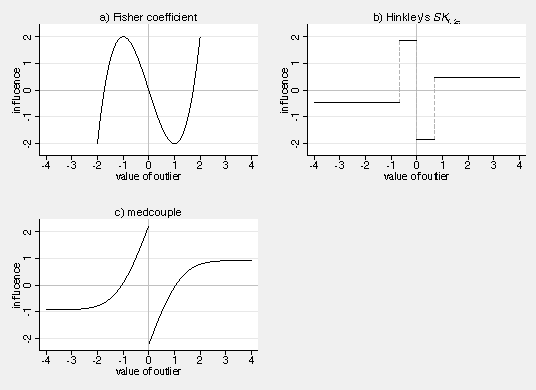
\epsfig{file=eps/3/4,width=.9\textwidth}
    \caption{Influence functions of $\gamma_1$, $\stsc{SK}_{0.25}$ and $\stsc{MC}$ under the standard normal distribution}
    \label{fig:stat:IF_skew}
\end{figure}

\subsection{Yule and Kendall, and Hinkley skewness measures}
\index{subject}{Yule and Kendall skewness|(textbf}
\index{subject}{Hinkley skewness|(textbf}

Alternative estimators of skewness, such as $(\mu_n-\text{mode}_n)/\sigma_n$ 
and $(\mu_n-Q_{0.5;n})/\sigma_n$ as proposed by Karl Pearson,
are just as fragile with respect to outliers as the standard
skewness estimator. 

Fortunately, robust alternatives based on quantiles are
available. For example, Yule and Kendall have proposed the skewness measure     \todo{Do you have a citation for this?}
\[
    \stsc{SK}_{\stsc{YK}}
    = \frac{(Q_{0.75} - Q_{0.5}) - (Q_{0.5}-Q_{0.25})}{Q_{0.75} - Q_{0.25}}
    = \frac{Q_{0.25} + Q_{0.75} - 2Q_{0.5}}{Q_{0.75} - Q_{0.25}}
\]
where $Q_{0.25}$, $Q_{0.5}$, and $Q_{0.75}$ are the three quartiles.

\citet{hinkley:1975} generalized this formula to other quantiles:
\[
    \stsc{SK}_p 
    = \frac{(Q_{1-p} - Q_{0.5}) - (Q_{0.5} - Q_p)}{Q_{1-p} - Q_p}
    = \frac{Q_p + Q_{1-p} - 2Q_{0.5}}{Q_{1-p} - Q_p},
\]
where $Q_p$ and $Q_{1-p}$ are the quantiles of order $p$ and $1-p$ (with
$0<p<0.5$). Hinkley's measure $\stsc{SK}_p$ is equal to zero for symmetric
distributions, is positive for right tailed (left skewed) and negative for left
tailed (right skewed) distributions. It has a much smaller asymptotic variance
under the standard normal distribution than $\gamma_1$. For instance,
$\stsc{ASV}(\stsc{SK}_{0.25}, \Phi) = 1.8421$.                                  \todo{How is the ASV derived? Plus: what is the expected value of $Q_{0.25}$ for Gaussian data?}
The asymptotic breakdown point of $\stsc{SK}_p$ is equal to $100p\%$ (in
particular, the Yule and Kendall skewness estimator, corresponding to $p=0.25$,
has an asymptotic breakdown point equal to 25\%).

For a \emph{symmetric} distribution $F$ with density $f$ and, without loss of
generality, $\mu(F) = F^{-1}(0.5) = 0$ and $\sigma(F) = 1$, the influence
function of $\stsc{SK}_p$ is
\[
    \stsc{IF}(x; \stsc{SK}_p, F) =
    \begin{cases}
        \frac{-1 / f(0)}{F^{-1}(1-p) - F^{-1}(p)}                            & \text{if $0\leq x < F^{-1}(1-p)$} \\[1ex]
        \frac{1/f\left(F^{-1}(1-p)\right) - 1/f(0)}{F^{-1}(1-p) - F^{-1}(p)} & \text{if $F^{-1}(1-p)\leq x$}
    \end{cases}
\]
for $x \geq 0$ and $\stsc{IF}(x; \stsc{SK}_p, F) = -\stsc{IF}(-x;
\stsc{SK}_p, F)$ for $x<0$. The influence function for standard Gaussian data
is displayed in Figure~\ref{fig:stat:IF_skew}b. In case of an
\emph{asymmetric} distribution the influence function is much more complex
and is no longer an odd function of $x$ (see \citealp[p.~101]{groeneveld:1991}).

\index{subject}{Yule and Kendall skewness|)}
\index{subject}{Hinkley skewness|)}

\subsection{The medcouple}
\index{subject}{medcouple|(textbf}

As usual when working with quantiles, the influence function of $\stsc{SK}_p$
is not smooth. To tackle this problem, \citet{brys:etal:2004a} propose to
replace the quantiles $Q_p$ and $Q_{1-p}$ in $\stsc{SK}_p$ by actual data
points and introduce a new skewness measure called \emph{medcouple}. 
Let $x_{(1)}\leq x_{(2)}\leq\dots\leq x_{(n)}$ be the $n$ order
statistics associated to the sample $\stmat{X}_n$ and $Q_{0.5;n}$ be 
the sample median. The medcouple is then defined as
\[
    \stsc{MC}_n =\med_{x_{(i)} \leq Q_{0.5;n} \leq x_{(j)}} 
    h \left(x_{(i)}, x_{(j)}\right)
\]
where, for all $x_{(i)} \neq x_{(j)}$, the kernel function $h$ is given as
\[
    h\left(x_{(i)}, x_{(j)}\right) = 
    \frac{\left(x_{(j)} - Q_{0.5;n}\right) - \left(Q_{0.5;n} - x_{(i)}\right)}{x_{(j)}-x_{(i)}}
\]
For the special case $x_{(i)}=x_{(j)}=Q_{0.5;n}$, the kernel is defined as
follows: let $m_1 < \dots < m_{k}$ denote the indices of the order statistics
that are tied to the median $Q_{0.5;n}$ (that is $x_{(m_{l})}  =Q_{0.5;n}$ for
all $l=1,\dots,k$). Then,
\[
    h \left(x_{(m_i)}, x_{(m_j)}\right) =
    \begin{cases}
        -1  & \text{if $i+j<k+1$}\\
        0   & \text{if $i+j=k+1$}\\
        1   & \text{if $i+j>k+1$}\\
    \end{cases}
\]
Due to the denominator it is clear that $h\left(x_{(i)}, x_{(j)}\right)$, 
and hence $\stsc{MC}_n$, will always lie between $-1$ and $1$ (similar to
$\stsc{SK}_p$).

The functional form of the medcouple is simply defined at any continuous
distribution $F$ as 
\[
    \stsc{MC} = \stsc{MC}(F) = \med_{X \leq Q_{0.5} \leq Y} h(X,Y)
\]
where $Q_{0.5}=F^{-1}(0.5)$ is the median of $F$ and $X$ and $Y$ are i.i.d.
random variables of distribution $F$. The kernel $h$ is the same as above with
the finite-sample median $Q_{0.5;n}$ replaced by $Q_{0.5}$. This functional
$\stsc{MC}$ is equal to zero in case of a symmetric distribution $F$. It is
positive for right tailed (left skewed) and negative left tailed (right skewed)
distributions.

The asymptotic breakdown point of the medcouple is equal to 25\%, which is the
same as for the quartile skewness $\stsc{SK}_{0.25}=\stsc{SK}_\stsc{YK}$. 
The advantage of $\stsc{MC}$, however, lies in the fact that its
influence function resembles a smoothed version of the influence function
of $\stsc{SK}_p$ ($0<p<0.5$). In particular, for standard Gaussian $F$, the   \todo{Why $\stsc{SK}_p$? Why not $\stsc{SK}_{0.25}$?} 
influence function is given as
\[
    \stsc{IF}(x; \stsc{MC}, \Phi) = \pi \left(2\Phi(x) - 1 - \frac{\sign(x)}{\sqrt{2}}\right)
\]
(see Figure~\ref{fig:stat:IF_skew}c). This leads to an asymptotic variance for
Gaussian data of                                                                \todo{Is 1.25 an exact result? How do you compute that? Plus: what is the expected value of medcouple for Gaussian data?}
\[
    \stsc{ASV}(\stsc{MC}, \Phi) = \int_{-\infty}^{\infty} \stsc{IF}(x;\stsc{MC},\Phi)^2 \dif \Phi(x) = 1.25
\]


\index{subject}{medcouple|)}

\subsection{Summary}

Table \ref{tab:stat:skewness} provides an overview of the
properties of the discussed skewness estimators. As can be seen, both proposed
robust estimators are more robust and, at the same time, more efficient than 
the standard skewness coefficient.                                              \todo{How to compute efficiency? Need to rescale...}

\begin{table}[h!]
    \centering
    \caption{Characteristics of the three skewness estimators}
    \label{tab:stat:skewness}
    \begin{tabular}{lcccc}
        \toprule
        Estimator
        & Class  
        & \subtab{c}{Gaussian\\ efficiency\textsuperscript{\textit{a}}}
        & \subtab{c}{Asymptotic\\ breakdown\\ point} 
        & \subtab{c}{Bounded\\ influence\\ function}
        \\\midrule
        Fisher coefficient $\gamma_{1;n}$     & moment   & 100\%        &  0\% & no
        \\\addlinespace
        Hinkley's $\stsc{SK}_{0.25;n}$      & quantile & \alert{???} & 25\% & yes
        \\\addlinespace
        medcouple $\stsc{MC}_n$             & pairwise & \alert{???} & 25\% & yes
        \\\bottomrule
        \multicolumn{5}{l}{\footnotesize\textsuperscript{\textit{a}} relative to the 
        efficiency of the Fisher coefficient}
    \end{tabular}
\end{table}

\index{subject}{skewness estimators|)}

\section{Robust estimation of the tails heaviness}
\label{subsec:kurtosis}
\index{subject}{kurtosis estimators|(textbf}

\subsection{The classical kurtosis coefficient}

The classical \emph{kurtosis coefficient} is defined by the functional
\[
    \gamma_2 = \gamma_2(F) = \mu_{4}(F)/\sigma(F)^{4}
\]
with
\[
    \mu_{4}(F) = \int_{-\infty}^\infty \left(x-\mu(F)\right)^{4} \dif F(x)
\]
Given a sample $\stmat{X}_n$, $\gamma_{2;n}$ is computed as
\[
    \gamma_{2;n} = \frac{1}{n} \sum_{i=1}^n \left(\frac{x_i-\mu_n}{\sigma_n}\right)^{4}
\]
with $\mu_n$ and $\sigma_n$ as the sample \Index{mean} and the \Index{standard
deviation}. 

The kurtosis coefficient is often considered as a measure of the
tail heaviness of a distribution relative to that of the normal distribution.
In particular, $\gamma_2$ is equal to three in case of distributions with a
tails heaviness similar to the normal distribution, is larger than three for
leptokurtic distributions (i.e., distributions with heavier tails than the
normal distribution) and is smaller than three for platokurtic distributions
(i.e., distributions with lighter tails than the normal distribution).
However, since the coefficient also measures the peakedness of a
distribution, there is no agreement on what the kurtosis really estimates. Another
disadvantage of the kurtosis is that its interpretation, and consequently its
use, is restricted to symmetric distributions (due of its intrinsic
comparison with the symmetric normal distribution). Moreover, as usual for
estimators relying on the mean and the standard deviation, the kurtosis
coefficient is very sensitive to outliers in the data. This is reflected in
the asymptotic breakdown point being equal to zero. The influence function is unbounded 
and is given as
\[
    \stsc{IF}(x; \gamma_2,F) = (z^2-\gamma_2)^2 - \gamma_2(\gamma_2-1) - 4\gamma_1 z,
\]
where $z = \left(x-\mu(F)\right)/\sigma(F)$, $\gamma_1 = \mu_{3}(F)/\sigma(F)^{3}$ and
$\gamma_2 = \mu_{4}(F)/\sigma(F)^{4}$ (see \citealp{ruppert:1987}).
See Figure~\ref{fig:stat:IF_tail}a for a graphical display of the influence function for 
standard Gaussian $F$, which is given as $\stsc{IF}(x; \gamma_2, \Phi) = (x^2-3)^2-6$.
The form of the influence function indicates that contamination
at the center has far less influence than that in the extreme tails. This
suggests that $\gamma_2$ is primarily a measure of tail behavior, and only
to a lesser extent of peakedness. The asymptotic variance of $\gamma_2$ for Gaussian 
data is given as $\stsc{ASV}(\gamma_2, \Phi) = 24$.                           \todo{Closed form solution?}



\begin{figure}[h!]
    \centering
    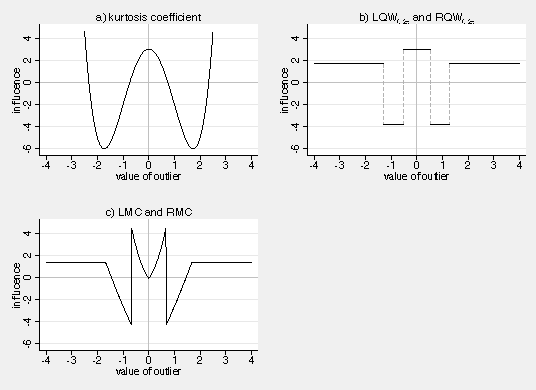
\epsfig{file=eps/3/5,width=.9\textwidth}
    \caption{Influence functions of $\gamma_2$, $\stsc{LQW}_{0.25}$ and $\stsc{RQW}_{0.25}$, $\stsc{LMC}$ and $\stsc{RMC}$ under the standard normal distribution}
    \label{fig:stat:IF_tail}
\end{figure}

\subsection{The quantile and medcouple tail weight measures}

To overcome the problems of the kurtosis coefficient, \citet{brys:etal:2006}
have proposed two measures of \emph{left} and \emph{right} tail weight for
univariate continuous distributions. As discussed below, these measures have
the advantage that they can be applied to symmetric as well as asymmetric
distributions that do not need to have finite moments. Moreover, their
interpretation is unambiguous and they are robust against outlying values.

More precisely, \citet{brys:etal:2006} defined \emph{left} and \emph{right}
tail measures as measures of skewness that are applied to the half of the
probability mass lying on the left side or on the right side of the median
$Q_{0.5}$ of the distribution $F$, respectively. As candidate measures of skewness 
they use both, $\stsc{SK}_p$ ($0<p<0.5$) and $\stsc{MC}$ (see above).

Recall that $\stsc{SK}_p$ is a measure of skewness of the distribution $F$
around $Q_{0.5}$, involving the quantiles $Q_p$ and $Q_{1-p}$ of orders $p$
and $(1-p)$ of $F$. Applying $-\stsc{SK}_{p/2}$ to the left half of the
distribution $F$ (i.e., to $x<Q_{0.5}$) leads to the \emph{Left Quantile
Weight} $\stsc{LQW}_p = \stsc{LQW}_p(F)$, which corresponds to (the
opposite of) a measure of skewness of the left half of $F$ around the first
quartile $Q_{0.25}$ involving the quantiles $Q_{p/2}$ and $Q_{0.5-p/2}$:
\[
    \stsc{LQW}_p 
    = -\frac{(Q_{0.5-p/2} - Q_{0.25}) - (Q_{0.25} - Q_{p/2})}{Q_{0.5-p/2}-Q_{p/2}}
    = -\frac{Q_{p/2}  +Q_{0.5-p/2} - 2 Q_{0.25}}{Q_{0.5-p/2} - Q_{p/2}}.
\]
Similarly, applying $\stsc{SK}_{p/2}$ to the right half of the distribution
$F$ (i.e., to $x>Q_{0.5}$) provides the \emph{Right Quantile Weight}
$\stsc{RQW}_p = \stsc{RQW}_p(F)$ which corresponds to a measure of
skewness of the right half of $F$ around the third quartile $Q_{0.75}$
involving the quantiles $Q_{0.5+p/2}$ and $Q_{1-p/2}$:
\[
    \stsc{RQW}_p
    = \frac{(Q_{1-p/2} - Q_{0.75}) - (Q_{0.75} - Q_{0.5+p/2})}{Q_{1-p/2} - Q_{0.5+p/2}}
    = \frac{Q_{0.5+p/2} + Q_{1-p/2} - 2 Q_{0.75}}{Q_{1-p/2} - Q_{0.5+p/2}}.
\]
With $p = 1/4 = 0.25$, we obtain
%
\begin{align*}
    \stsc{LQW}_{0.25} & = -\frac{Q_{0.125} + Q_{0.375} - 2 Q_{0.25}}{Q_{0.375} - Q_{0.125}}\\[1ex]
    \stsc{RQW}_{0.25} & =  \frac{Q_{0.625} + Q_{0.875} - 2 Q_{0.75}}{Q_{0.875} - Q_{0.625}}
\end{align*}
%
Note that the sample versions $\stsc{LQW}_{p;n}$ and $\stsc{RQW}_{p;n}$
are easily found by using the quantiles of $F_n$, the empirical distribution
function of $\stmat{X}_n$.

As with $\stsc{LQW}$ and $\stsc{RQW}$, we can also apply the $\stsc{MC}$ to
each side of the distribution, leading to the \emph{Left Medcouple}
($\stsc{LMC}$) and to the \emph{Right Medcouple} ($\stsc{RMC}$), defined
as
%
\begin{align*}
    \stsc{LMC} &=\stsc{LMC}(F) = -\stsc{MC}(x<Q_{0.5})\\[1ex]
    \stsc{RMC} &=\stsc{RMC}(F) = \stsc{MC}(x>Q_{0.5})
\end{align*}
%
By using $\stsc{MC}_n$, the finite-sample version of $\stsc{MC}$, we
obtain the finite-sample versions $\stsc{LMC}_n$ and $\stsc{RMC}_n$.

Since both the quantile and the medcouple tail weight measures only depend on
quantiles, they are given for any distribution, even for distributions without
finite moments. Note that $\stsc{LQW}$ and $\stsc{RQW}$ require to fix the
parameter $p$ in advance (depending on the degree of robustness one wants to
attain), whereas $\stsc{LMC}$ and $\stsc{RMC}$ do not require any
additional parameter to be set.

Some general properties of the tail weight measures are as follows. 
Let $X$ be a random variable with continuous distribution $F_X$. Furthermore, 
let $\stsc{W}$ stand for any of the defined tail weight measures; 
let $\stsc{LW}$ stand for left tailed measures and $\stsc{RW}$ 
for the right tailed measures. Then:
\begin{itemize}
    \item Like the skewness measures $\stsc{SK}_p$ and $\stsc{MC}$,
    $\stsc{W}$ is location and scale invariant. That is, $\stsc{W}(F_{aX+b}) = \stsc{W}(F_X)$.

    \item $\stsc{LW}(F_{-X}) = \stsc{RW}(F_X)$.

    \item If $F$ is symmetric, then $\stsc{LW}(F) = \stsc{RW}(F)$.

    \item $\stsc{W} \in[-1,1]$.
\end{itemize}

The medcouple tail weight measures can resist up to 12.5\% outliers in the
data. In a similar way, it can be shown that the left and right quantile tail
weight measures $\stsc{LQW}_p$ and $\stsc{RQW}_p$ have an asymptotic
breakdown point equal to $(100p/2)\%$; in particular, $\stsc{LQW}_{0.25}$
and $\stsc{RQW}_{0.25}$ have the same asymptotic breakdown point as
$\stsc{LMC}$ and $\stsc{RMC}$, and $\stsc{LQW}_{0.125}$ and
$\stsc{RQW}_{0.125}$ have an asymptotic breakdown point of 6.25\%.

Moreover, the influence functions of $\stsc{LMC}$ and $\stsc{RMC}$ are
smooth versions of the influence functions of $\stsc{LQW}_{0.25}$ and
$\stsc{RQW}_{0.25}$, as shown in Figure~\ref{fig:stat:IF_tail}b and c for
standard Gaussian $F$.\footnote{Figure~\ref{fig:stat:IF_tail} shows only the
left part (defined on ${\mathbb{R}}^{-}$) of the influence functions of
$\stsc{LMC}$ and $\stsc{LQW}_{0.25}$, and the right part (defined on
${\mathbb{R}}^{+}$) of the influence functions of $\stsc{RMC}$ and
$\stsc{RQW}_{0.25}$.} All these influence functions are bounded. More
precisely, if $F$ is a continuous distribution with density $f$ and if we
denote, as usual, the quantile of order $p$ of $F$ by $Q_p=F^{-1}(p)$, we have
\[
    \stsc{IF}(x; \stsc{LQW}_p, F) 
         = 2\, \frac{\begin{array}{@{}l@{}}
                    \left(\stsc{IF}(x; Q_{0.25}, F) - \stsc{IF}(x; Q_{0.5-p/2}, F)\right)
                                       \left(q_{0.25} - Q_{p/2}\right)\\
                    \qquad - \left(\stsc{IF}(x; Q_{p/2}, F) - \stsc{IF}(x;Q_{0.25},F)\right) 
                                       \left(Q_{0.5-p/2} - Q_{0.25}\right)
                    \end{array}}
            {\left(Q_{0.5-p/2} - Q_{p/2}\right)^2}
\]
and
\[
    \stsc{IF}(x; \stsc{RQW}_p, F) 
         = 2\, \frac{\begin{array}{@{}l@{}}
                    \left(\stsc{IF}(x; Q_{0.5+p/2}, F) - \stsc{IF}(x; Q_{0.75}, F)\right)
                                       \left(q_{1-p/2} - Q_{0.75}\right)\\
                    \qquad - \left(\stsc{IF}(x; Q_{0.75}, F) - \stsc{IF}(x;Q_{1-p/2},F)\right) 
                                       \left(Q_{0.75} - Q_{0.5+p/2}\right)
                    \end{array}}
            {\left(Q_{1-p/2} - Q_{0.5+p/2}\right)^2}
\]
with 
\[
    \stsc{IF}(x; Q_p, F) = \frac{p - \I[x<Q_p]}{f(Q_p)}
\]
The expression of the influence functions of $\stsc{LMC}$ and $\stsc{RMC}$
is more complex and can be found in \citet[p.~740--741]{brys:etal:2006}.        \todo{(maybe have a look and then 
                                                                                check computation of graph; it seems IF
                                                                                has a discontinuity; need to use shortdash)}

Finally, the asymptotic variances of the left and right tail weight measures    
under Gaussian distributions are much smaller than the variance of the classical
kurtosis coefficient $\gamma_2$. In particular:                                 \todo{How are these numbers computed? Furthermore,
                                                                                is it a fair comparison. That is, are L/RQW and L/RMC
                                                                                similar in size to the kurtosis for Gaussian data or
                                                                                do they have to be rescaled? Only if the measures 
                                                                                have the same size the variances can be compared.}
%
\begin{align*}
    \stsc{ASV}(\stsc{LQW}_{0.25}, \Phi)   & = \stsc{ASV}(\stsc{RQW}_{0.25}, \Phi)  = 3.71 \\
    \stsc{ASV}(\stsc{LQW}_{0.125}, \Phi)  & = \stsc{ASV}(\stsc{RQW}_{0.125}, \Phi) = 2.23
\end{align*}
%
and
\[
    \stsc{ASV}(\stsc{LMC}, \Phi)  = \stsc{ASV}(\stsc{RMC}, \Phi) = 2.62
\]


\subsection{Summary}

Table \ref{tab:stat:kurt} summarizes the properties of the presented tails
heaviness estimators. \alert{[Another sentence needed here!]}           \todo{How to compute efficiency? (need to rescale)}

\begin{table}[h!]
    \centering
    \caption{Characteristics of the three tails heaviness estimators}
    \label{tab:stat:kurt}
    \begin{tabular}{lcccc}
        \toprule
        Estimator
        & Class  
        & \subtab{c}{Gaussian\\ efficiency\textsuperscript{\textit{a}}}
        & \subtab{c}{Asymptotic\\ breakdown\\ point} 
        & \subtab{c}{Bounded\\ influence\\ function}
        \\\midrule
        kurtosis coefficient $\gamma_{2;n}$                  & moment   & 100\%        &  0\% & no
        \\\addlinespace
        $\stsc{LQW}_{0.25;n}$ and $\stsc{RQW}_{0.25;n}$      & quantile & \alert{???} & 12.5\% & yes
        \\\addlinespace
        $\stsc{LMC}_n$ and $\stsc{RMC}_n$                    & pairwise & \alert{???} & 12.5\% & yes
        \\\bottomrule
        \multicolumn{5}{l}{\footnotesize\textsuperscript{\textit{a}} relative to the 
        efficiency of the kurtosis coefficient}
    \end{tabular}
\end{table}

\index{subject}{kurtosis estimators|)}

\section{Example}                                                               \todo{The examples will be replaced 
                                                                                later by the \stcmd{robstat} command. 
                                                                                Possibly, it would be good to split 
                                                                                the example into parts and include the
                                                                                parts at appropriate placed in the 
                                                                                sections above.}

As an illustrative example we will generate two datasets (of size $n = 1000$),
one drawn from a standard normal distribution and one drawn from a chi-square
distribution with one degree of freedom. All descriptive statistics presented
above will be calculated for both samples. To simplify interpretation we will
present the excess kurtosis rather than the kurtosis (in other words, the
reported tail heaviness statistics are equal to zero for the normal
distribution). We then contaminate the datasets by replacing a random selection
of 5\% of the observations by value 5 for the normally distributed sample and
by $F_{\chi_1^2}^{-1}(\Phi(5))$ for the chi-square distributed sample,
$F_{\chi_1^2}^{-1}$ and $\Phi$ are the quantile function of the $\chi_1^2$
distribution and the normal cumulative distribution function, respectively. In
this way the degree of outlyingness is comparable between the two setups.

When we compare the classical, quantile-based and pairwise-based estimates
obtained for the normally distributed dataset free of outliers (see the upper
part of table~\ref{tab:clear_samples_estimates}), we do not see big differences
between the three types of approaches. Indeed, the estimates all point towards
a symmetrical distribution centered at zero with non-excessive tails and a
dispersion of about one. If one looks at these statistics for the case of the
chi-squared distributed data (see the lower part of
table~\ref{tab:clear_samples_estimates}), the location estimate is, as
expected, not the same since the mean is more attracted by the tail than the
robust competitors. A similar phenomenon occurs for skewness and tails
heaviness.

\begin{table}[h!]
    \centering
    \caption{The estimates of location, scale, skewness and tails heaviness in 
    the original (uncontaminated) datasets}
    \label{tab:clear_samples_estimates}
    \begin{tabular}[c]{l*{5}{D{.}{.}{2.3}}}
        \toprule
                        &&&& \multicolumn{2}{c}{Tails heaviness}
                        \\\cmidrule(lr){5-6}
                        & \multicolumn{1}{c}{Location}
                        & \multicolumn{1}{c}{Scale}
                        & \multicolumn{1}{c}{Skewness}
                        & \multicolumn{1}{c}{Left} 
                        & \multicolumn{1}{c}{Right}
                        \\
        \midrule
        \textit{Normally distributed sample}                                            \\
        Classical       & 0.015     & 0.977     & -0.006    & \multicolumn{2}{c}{0.157} \\
        Quantile-based  & 0.031     & 0.946     & -0.088    & 0.025     & 0.0139        \\
        Pairwise-based  & 0.017     & 0.973     & -0.024    & 0.038     & 0.075         \\
        \addlinespace
        \textit{Chi-square distributed sample}                                          \\
        Classical       & 0.993     & 1.406     & 2.322     & \multicolumn{2}{c}{6.323} \\
        Quantile-based  & 0.414     & 0.908     & 2.491     & -0.439    & 0.135         \\
        Pairwise-based  & 0.652     & 0.496     & 0.539     & -0.491     & 0.190        \\
        \bottomrule
    \end{tabular}
\end{table}

When the dataset is contaminated by a small portion of outliers, the classical
statistics change substantially, while the effect on their robust equivalent is
only marginal (table~\ref{tab:contaminated_samples_estimates}). For example,
for the normal case, classical statistics would point towards a right-tailed
skewed distribution with relatively large dispersion and big-tail heaviness.
The robust counterparts would still point towards the standard normal
distribution. A similar phenomenon is observable for the chi-square.

\begin{table}[h!]
    \centering
    \caption{The estimates of location, scale, skewness and tails heaviness in 
    the contaminated datasets}
    \label{tab:contaminated_samples_estimates}
    \begin{tabular}[c]{l*{5}{D{.}{.}{2.3}}}
        \toprule
                        &&&& \multicolumn{2}{c}{Tails heaviness}
                        \\\cmidrule(lr){5-6}
                        & \multicolumn{1}{c}{Location}
                        & \multicolumn{1}{c}{Scale}
                        & \multicolumn{1}{c}{Skewness}
                        & \multicolumn{1}{c}{Left} 
                        & \multicolumn{1}{c}{Right}
                        \\
        \midrule
        \textit{Normally distributed sample}                                            \\
        Classical       & 0.263     & 1.447     & 1.530     & \multicolumn{2}{c}{3.465} \\
        Quantile-based  & 0.086     & 1.012     & 0.016     & 0.023     & 0.055         \\
        Pairwise-based  & 0.109     & 1.072     & 0.041     & 0.030     & 0.145         \\
        \addlinespace
        \textit{Chi-square distributed sample}                                          \\
        Classical       & 1.011     & 1.416     & 2.311     & \multicolumn{2}{c}{6.276} \\
        Quantile-based  & 0.437     & 0.923     & 2.305     & -0.458    & 0.135         \\
        Pairwise-based  & 0.672     & 0.518     & 0.522     & -0.492    & 0.189         \\
        \bottomrule
    \end{tabular}
\end{table}

\alert{
\begin{stlog}
. robreg lts log_light log_temp
{\smallskip}
enumerating 500 samples (percent completed)
0 \HLI{5} 20 \HLI{6} 40 \HLI{6} 60 \HLI{6} 80 \HLI{5} 100
..................................................
{\smallskip}
LTS regression                                  Number of obs     =         47
                                                  Breakdown point =         .5
                                                  Subsamples      =        500
                                                  Scale estimate  =  .40961741
{\smallskip}
\HLI{13}{\TOPT}\HLI{64}
   log_light {\VBAR}      Coef.
\HLI{13}{\PLUS}\HLI{64}
    log_temp {\VBAR}   4.727267
       _cons {\VBAR}  -15.81634
\HLI{13}{\BOTT}\HLI{64}
{\smallskip}

\end{stlog}
}

\section{Robust tests of normality}

The estimates of location, scale, skewness and tails heaviness can be used to
characterize the underlying distribution. In particular, they can be used to
test for normality. For example, \citet{Jarque:Bera:1980} have proposed a
normality test relying on the classical skewness and kurtosis coefficients.
More precisely, under the normality assumption ($\gamma_1=0$ and $\gamma_2=3$),
we have
\[ 
    \sqrt{n}
    \begin{bmatrix}
        \gamma_{1;n} \\
        \gamma_{2;n} - 3
    \end{bmatrix}
    \stackrel{d}{\rightarrow}
    \mathcal{N}\left(
    \begin{bmatrix}
        0 \\
        0
    \end{bmatrix},
    \begin{bmatrix}
        6 & 0\\
        0 & 24
    \end{bmatrix}
    \right)
\]
which leads to the Jarque-Bera test statistic
\[
    T = n \left(\frac{\gamma_{1;n}^2}{6} + 
          \frac{\left(\gamma_{2;n} - 3\right)^2}{24}\right)
    \approx \chi_2^2
\]

The Jarque-Bera test is a very popular and interesting test for normality. It
has been shown that, for a wide range of alternative distributions, it
outperforms tests such as the Kolmogorov-Smirnov test, the Cramér-von Mises
test and the Durbin test. Unfortunately, despite its good power properties and
computational simplicity, the Jarque-Bera test is highly sensitive to outliers
because it is constructed from the moment-based skewness and kurtosis measures.

Robust alternatives to the Jarque-Bera test have been proposed and studied in
\citet{brys:etal:2004b}. The authors start from the fact that the Jarque-Bera
test can be seen as a special case of the following general testing procedure.
Let $\sthat{\boldsymbol\theta} = (\sthat{\theta}_1, \dots, \sthat{\theta}_p)'$
be a vector of estimators of $\boldsymbol\theta = (\theta_1, \dots, \theta_p)'$
(a vector of characteristic parameters of the underlying distribution) such
that, under the null hypothesis of normality,
\[
    \sqrt{n} \left(\sthat{\boldsymbol\theta} - \boldsymbol{\theta}\right)'
    \stackrel{d}{\rightarrow}
    \mathcal{N}(\stvec{0},\boldsymbol\Omega)
\]
Then, the general test consists in rejecting, at level $\alpha$, the null
hypothesis of normality if
\[
    T = n\left(\sthat{\boldsymbol\theta} - \boldsymbol\theta\right)'
    \boldsymbol\Omega^{-1}
    \left(\sthat{\boldsymbol\theta} - \boldsymbol\theta\right)
    > \chi_{p;1-\alpha}^2
\]
where $\chi_{p;1-\alpha}^2$ is the $(1-\alpha)$-quantile of the chi-square
distribution with $p$ degrees of freedom. \citet{brys:etal:2004b} then propose
to use, in this general testing procedure, the robust skewness estimator
$\stsc{MC}_n$ or the tails heaviness estimators $\stsc{LMC}_n$ and
$\stsc{RMC}_n$.

Three tests have been studied. The first one is only based on the skewness
estimator $\stsc{MC}_n$ (the medcouple). In this case, $k=1$, $\sthat{\theta} =
\stsc{MC}_n$ and $\Omega = 1.25$. The second one is based on the left and right
tail heaviness estimators $\stsc{LMC}_n$ (left medcouple) and $\stsc{RMC}_n$
(right medcouple). In this case, $k=2$, $\sthat{\boldsymbol\theta} =
(\stsc{LMC}_n, \stsc{RMC}_n)'$, $\boldsymbol\theta = (0.199, 0.199)'$ and
\[
    \boldsymbol\Omega = 
    \begin{bmatrix}
        2.62    & -0.0123\\
        -0.0123 & 2.62
    \end{bmatrix}
\]
The third test combines $\stsc{MC}_n$, $\stsc{LMC}_n$ and $\stsc{RMC}_n$. In
this case, $k=3$, $\sthat{\boldsymbol\theta} = (\stsc{MC}_n, \stsc{LMC}_n,
\stsc{RMC}_n)'$, $\boldsymbol\theta = (0, 0.199, 0.199)'$ and
\[
    \boldsymbol\Omega =
    \begin{bmatrix}
        1.25   & 0.323   & -0.323  \\
        0.323  & 2.62    & -0.0123 \\
        -0.323 & -0.0123 & 2.62
    \end{bmatrix}
\]
This last test seems to have the best overall performance.

\begin{stexample}                                                               \todo{The example will be revised to 
                                                                                so that the relevant Stata code is 
                                                                                visible.}
We will analyze the body weight of 64 different animal species. The dataset we
use is available online.\footnote{See
\url{http://onlinestatbook.com/stat\_sim/transformations/body\_weight.html}}
These data have been made available by Rice University, University of Houston
Clear Lake and Tufts University.

To start the analysis, we first calculate the classic estimators of
location, scale, skewness and kurtosis using Stata's \stcmd{summary} command
with the \stcmd{detail} option. The results are presented in the first line
of Table~\ref{tab:estimates_original_data}. In the second line of the table we
present the results obtained using the commands for robust estimators (that is,
\stcmd{hl}, \stcmd{qn}, \stcmd{medcouple} and \stcmd{medcouple} with the
\stcmd{lmc} and \stcmd{rmc} options).

\begin{table}[h!]
    \centering
    \caption{Classic estimates of location, scale, skewness and tails heaviness
    as well as estimates based on pairwise combinations}
    \label{tab:estimates_original_data}
    \begin{tabular}{lcccc}
        \toprule
                  & Location 
                  & Dispersion 
                  & Skewness 
                  & Tails
        \\\midrule
        Classic   & $\mu_n          = \numprint{3111355}$ 
                  & $\sigma_n       = \numprint{1.3e7}$ 
                  & $\gamma_{1;n}   = \numprint{5.461}$ 
                  & $\gamma_{2;n}   = \numprint{32.77}$
        \\\addlinespace
        Robust    & $Q_{0.5;n}      = \numprint{3500}$
                  & $Q_n            = \numprint{6667.5}$
                  & $\stsc{MC}_n    = \numprint{0.985}$
                  & $\stsc{LMC}_n   = \numprint{-0.090}$
        \\
                  & $\stsc{HL}_n    = \numprint{94307}$
                  &
                  &
                  & $\stsc{RMC}_n   = \numprint{0.915}$
        \\\bottomrule
    \end{tabular}
\end{table}

If we would only look at the classic estimators, we would conclude that the
average animal weight is very high, but with a huge dispersion. The asymmetry
is large and positive and tails are very heavy. When we look at the equivalent
robust statistics, we see that the median weight is much lower than the mean
weight. The robust dispersion is also much smaller than that suggested by the
standard deviation and right skewness is extreme. As far as the heaviness of
the tails is concerned, the right tail is extremely heavy while the left one is
similar to the left tail of the normal (even slightly lighter). When looking at
the difference between classical and robust estimators, it is evident that
outliers are present in the dataset.

A first way to tackle this problem is to transform the data to reduce the
excessive importance of very big animals (such as dinosaurs). Given that
weights are strictly positive, we consider a logarithmic transformation and
redo the above descriptive statistics analysis (see
Table~\ref{tab:estimates_transformed_data}).


\begin{table}[h!]
    \centering
    \caption{Classic estimates of location, scale, skewness and tails heaviness
    as well as estimates based on pairwise combinations based on transformed data}
    \label{tab:estimates_transformed_data}
    \begin{tabular}{lcccc}
        \toprule
                  & Location 
                  & Dispersion 
                  & Skewness 
                  & Tails
        \\\midrule
        Classic   & $\mu_n          = \numprint{9.313}$ 
                  & $\sigma_n       = \numprint{4.135}$ 
                  & $\gamma_{1;n}   = \numprint{0.304}$ 
                  & $\gamma_{2;n}   = \numprint{2.192}$
        \\\addlinespace
        Robust    & $Q_{0.5;n}      = \numprint{8.161}$
                  & $Q_n            = \numprint{4.281}$
                  & $\stsc{MC}_n    = \numprint{0.386}$
                  & $\stsc{LMC}_n   = \numprint{0.515}$
        \\
                  & $\stsc{HL}_n    = \numprint{9.289}$
                  &
                  &
                  & $\stsc{RMC}_n   = \numprint{0.241}$
        \\\bottomrule
    \end{tabular}
\end{table}

When we do this transformation, we see that the differences between classic
and robust estimators become much smaller. Indeed the mean is only slightly
larger than the median, the dispersion estimate is very similar for both
methods as well as the skewness estimate that only points towards evidence of
very moderate positive skewness. As far as the heaviness of the tails is
concerned, the classic estimator is close to 3 which is the value of the
kurtosis of the normal distribution and therefore points towards standard tails.
Nevertheless when we look at the robust estimate for the latter, there is
evidence of a heavy left tail. This last point is very important.

The classic and the robust tests for the normality of the log-transformed body
weight variable lead to different findings. The standard Jarque-Bera statistic
is 2.726, which is much smaller than the critical value of $\chi_{2;0.95}^2 =
5.99$. That is, the standard Jarque-Bera test does not reject the null
hypothesis of normality. On the other hand, the robust test statistic involving
$\stsc{MC}_n$, $\stsc{LMC}_n$ and $\stsc{RMC}_n$ is equal to 9.266, which is
larger than the critical value of $\chi_{3;0.95}^2 = 7.815$. That is, the null
hypothesis of normality is rejected by the robust test. Even though the
logarithmic transformation substantially reduces the effect of atypical
observations, outliers still bias the classic test. In particular, we believe
that the heaviness of the left tail is not satisfactorily identified by the
classic kurtosis coefficient, and this affects the result of the normality test.
\end{stexample}



\section{Robust boxplots}

As stated by \citet{Bruffaerts:etal:2014}, among others, the boxplot is without
any doubt the most commonly used tool to represent the distribution of the data
and identify atypical observations in a univariate dataset. An observation is
considered as atypical (or extreme) when it is above the upper whisker or below
the lower whisker. An important issue with the standard boxplot is that, as
soon as asymmetry or tail heaviness appears, the percentage of values
identified as atypical becomes excessive. To cope with this,
\citet{hubert:vandervieren:2008} proposed an \emph{adjusted} boxplot for skewed
data. Their idea is to modify the whiskers according to the degree of asymmetry
in the data, which can be robustly measured by the medcouple. Alternatively,
\citet{Bruffaerts:etal:2014} propose to apply a simple rank-preserving
transformation on the original data so that the transformed observations can be
adjusted by a so-called \emph{Tukey g-and-h distribution}. Using the quantiles
of this distribution, it is then relatively easy to recover whiskers of the
boxplot related to the original data. Given the result of simulations, the
latter seems to be more efficient and we therefore concentrate on that too here.

\subsection{The classic boxplot and the adjusted boxplot}

In a univariate setup, an observation is often considered as atypical as soon
as its value does not belong to the interval $[Q_{0.25} - 1.5\,\stsc{IQR};
Q_{0.75} + 1.5\,\stsc{IQR}]$, where $Q_{0.25}$ and $Q_{0.75}$ are the first and
third quartiles, and $\stsc{IQR}$ is the interquartile range. For Gaussian
data, approximately 0.7\% of the observations will lie outside this interval.
Unfortunately, as soon as asymmetry or tail heaviness appears, the percentage
of values detected as atypical becomes excessively high. To deal with the above
drawbacks of the standard boxplot, \citet{hubert:vandervieren:2008} suggested
to use an alternative boxplot, called the adjusted boxplot, where the interval
for the boxplot is
\[
    \left[Q_{0.25} - 1.5 e^{-4\,\stsc{MC}} \stsc{IQR},\,
          Q_{0.75} + 1.5 e^{3\,\stsc{MC}} \stsc{IQR}\right] \quad \text{if $\stsc{MC} \geq 0$}
\]
and 
\[
    \left[Q_{0.25} - 1.5 e^{-3\,\stsc{MC}} \stsc{IQR},\,
    Q_{0.75} + 1.5e^{4\,\stsc{MC}} \stsc{IQR}\right] \quad \text{if $\stsc{MC} < 0$}
\]
where $\stsc{MC}$ is the medcouple.

Although this rule works well for most commonly used distributions, it presents
some limitations and drawbacks (see \citealp{Bruffaerts:etal:2014}), the most
restrictive probably being that it does not deal with excessive tail heaviness.
\citet{Bruffaerts:etal:2014} deal with most of these limitations. Since this
method relies on the Tukey $g$-and-$h$ distribution, we briefly describe this
distribution before explaining the methodology of \citet{Bruffaerts:etal:2014}.

\subsection{The Tukey $g$-and-$h$ distribution}

The Tukey $g$-and-$h$ family of distributions covers a large variety of
distributions which can substantially differ from normality in both skewness
and heaviness of the tails. If $Z$ is a random variable with standard normal
distribution, and $g$ and $h$ are two constants ($g \neq 0$, $h \in
\mathbb{R}$), then the random variable $Y$ given by
\[
    Y = \frac{1}{g} \left(\exp(g Z) - 1\right) \exp(h Z^2/2)
\]
is distributed as a Tukey $g$-and-$h$ distribution, that is $Y \sim
T(g,h)$.\footnote{Note that $Y$ is a strictly increasing transformation of
$Z$, driven by the values of $g$ and $h$. Hence, for every order $p \in (0,
1)$, $y_p = \frac{1}{g} \left(\exp(g z_p) - 1\right) \exp(h z_p^2/2)$, where
$y_p$ and $z_p$ are the quantiles of order $p$ of the distributions of $Y$ and
$Z$ respectively. This implies in particular that the median $y_{0.5}$ of $Y$
is equal to zero.} The constants $g$ and $h$ control the skewness and the tail
weight (or elongation) of the distribution, respectively. They can be estimated
from the empirical quantiles\footnote{The expression $Q_p(\{y_j\})$ denotes the
empirical quantile of order $p$ related to the series $\{y_1, \dots, y_n\}$.
The notation $\min(\{x_j\})$ and $\max(\{x_j\})$ is later used to define the
minimum and maximum values of the series $\{x_1, \dots, x_n\}$.}                \todo{Why such complicated notation?}
$Q_{1-p}(\{y_j\}) $ and $Q_p(\{y_j\})$ of order $(1-p)$ and $p$ ($0.5 < p < 1$)
of $n$ independent realizations $\{y_1, \dots, y_n\}$ of $Y$ (see
\citealp{Jimenez:2011}). Following \citet{Jimenez:2011}, $g$ and $h$ can be
estimated as follows:
%
\begin{equation}\label{eq:ghat_hhat}
    \sthat{g} = \frac{1}{z_p} \ln\left(-\frac{Q_p(\{y_j\})}{Q_{1-p}(\{y_j\})}\right)
    \qquad\text{and}\qquad
    \sthat{h} = \frac{2\ln\left(-\sthat{g}\, \frac{Q_p(\{y_j\}) Q_{1-p}(\{y_j\})}
                {Q_p(\{y_j\}) + Q_{1-p}(\{y_j\})}\right)}{z_p^2}
\end{equation}
%
where $z_p$ is the quantile of order $p$ of the standard normal distribution.
Note that the chosen order $p$ for the quantiles determines the robustness of
the method with respect to outliers. For example, if we set $p = 0.9$, the
breakdown point of the estimators of $g$ and $h$ is set to $1 - p = 10\%$, as
the method provides meaningful results if there are up to 10\% of outliers. For
estimation purposes, we suggest using $p = 0.9$, except if one believes that
the contamination rate is larger than 10\%. Working with a lower value for $p$
would increase robustness with respect to outliers, but at the cost of lowering
the efficiency. Furthermore, it would not make sense to work with a $p \leq
0.75$, as a contamination of more than 25\% would make the first and/or third
quartile of the boxplot break down.

\subsection{A generalized boxplot}

The method proposed by \citet{Bruffaerts:etal:2014} overcomes most of the
limitations of the adjusted boxplot. Based on an initial 
dataset $\{x_1, \dots, x_n\}$, their procedure is as follows. 

\begin{enumerate}
    \item Reduce the data by a scale factor $s_0$:
    \[
        x^*_i = \frac{x_i}{s_0}, \quad i= 1, \dots, n
    \]
    with $s_0 = \stsc{IQR}(\{x_j\})$, where $\stsc{IQR}(\{x_j\})$ is the
    interquartile range of the series $\{x_1, \dots, x_n\}$.

    \item Shift the dataset to obtain only strictly positive values: compute
    \[
        r_i = x^*_i - \min(\{x^*_j\}) + \zeta, \quad i= 1, \dots, n
    \]
    where $\zeta > 0$ is a small quantity. They propose to use $\zeta = 0.1$

    \item Standardize the values obtained in step 2 in order to obtain new values
    belonging to the open interval $(0,1)$: compute
    \[
        \widetilde{r}_i = \frac{r_i}{\min(\{r_j\})+ \max(\{r_j\})}, \quad i= 1, \dots, n
    \]

    \item Apply the inverse normal (probit) transformation
    \[
        w_i  =\Phi^{-1}(\widetilde{r}_i), \quad i= 1, \dots, n
    \]
     where $\Phi(\cdot)$ denotes the cumulative distribution
     function of the standard normal.

     \item Center and reduce the values $w_i$: compute
     \[
         w^*_i = \frac{w_i - Q_{0.5}(\{w_j\})}{\stsc{IQR}(\{w_j\})/1.3426}, 
         \quad i= 1, \dots, n
     \]
    where $Q_{0.5}(\{w_j\})$ and $\stsc{IQR}(\{w_j\})$ are the median and the
    interquartile range of the series $\{w_1,\dots, w_n\}$. The constant 1.3426
    ensures, in the Gaussian case, the consistency of the scale estimator
    $\stsc{IQR}(\{x_j\})$ with the scale parameter $\sigma$ (the standard
    deviation).

    \item Adjust the distribution of the values $w^*_i$, $i = 1, \dots, n$, by  \todo{I don't understand. What is exactly done in this step?}
    the Tukey $T(\sthat{g}^*,\sthat{h}^*)$ distribution, where $\sthat{g}^*$
    and $\sthat{h}^*$ are the estimates of the skewness and tail weight
    parameters $g$ and $h$ obtained by applying equation (\ref{eq:ghat_hhat})
    to the empirical quantiles $Q_{0.1}(\{w^*_j\})$ and $Q_{0.9}(\{w^*_j\})$ of
    orders 0.1 and 0.9 of the series $\{w^*_1, \dots, w^*_n\}$.

    \item Determine the quantiles $\xi^*_{\alpha/2}$ and $\xi^*_{1-\alpha/2}$ 
    of orders $\alpha/2$ and $1-\alpha/2$, $\alpha \in (0, 1)$, of the 
    $T_{\sthat{g}^*,\sthat{h}^*}$ distribution specified in the previous step, 
    where $\alpha$ corresponds to the desired detection rate of atypical values 
    in the absence of contamination with outliers. Let 
    \[
    \mathcal{I} = \left\{i=1, \dots, n 
        \left| w^*_i \notin \left[\xi^*_{\alpha/2},\, \xi^*_{1-\alpha/2}\right] \right.
        \right\}
    \] 
     be the set of indices of the values $w_i^{\ast}$ that are detected as
     atypical in the series $\{w^*_1, \dots, w^*_n\}$. The values $x_i$ for
     which $i \in \mathcal{I}$ are considered as atypical observations in the
     initial dataset.

     \item Based on the above steps, it is possible to come up with a
     \emph{generalized} boxplot which is associated to the original dataset.
     From the detection bounds $L^*_{-} = \xi^*_{\alpha/2}$ and $L^*_{+} =
     \xi^*_{1-\alpha/2}$ computed in step 7, one can build the respective
     detection bounds $B^*_{-}$ and $B^*_{+}$ for the related original dataset
     ($B^*_{-}$ and $B^*_{+}$ are the extremities of the lower and upper
     whiskers of the generalized boxplot):
     \begin{align*}
     B^*_{\pm} &= 
         \biggl(\Phi\left(Q_{0.5}(\{w_j\}) + \frac{\stsc{IQR}(\{w_j\})}{1.3426} L^*_{\pm}\right)
         \\
         &\quad \times \left\{\min(\{r_j\})+\max(\{r_j\})\right\}  + \min(\{x^*_j\}) - \zeta\biggr) s_0
     \end{align*}
\end{enumerate}


\begin{stexample}
We illustrate the use of the robust boxplot by an example from
\citealp{Bruffaerts:etal:2014}. The data contain daily earnings (in British
pounds) of 50 top soccer players.\footnote{Source:
\url{http://www.paywizard.co.uk/main/pay/vip-celebrity-salary/football-players-s
alary}} The left panel in Figure~\ref{fig:football} displays the kernel density
estimate of the earnings variable.\footnote{We use an Epanechnikov kernel with
Silverman's rule-of-thumb bandwidth.} The right panel displays the three
flavors of boxplots. Daily earnings appear to be slightly asymmetrically
distributed with a relatively heavy tail. A medcouple measure of 0.12 indicates
that the distribution is slightly asymmetric, but not too much. This explains
why the upper whisker of the generalized boxplot goes beyond the upper whisker
of the two other boxplots.
\end{stexample}


\begin{figure}[h!]
    \centering
    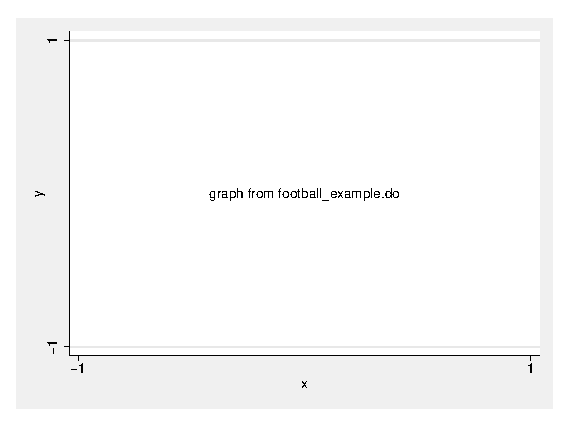
\epsfig{file=eps/3/7}
    \caption{Classic, adjusted, and generalized boxplot \alert{[will be inserted after revising the boxplot program]}}
    \label{fig:football}
\end{figure}
